
\chapter{核物理中的半经典方法\label{chap:=006838=007269=007406=004E2D=007684=00534A=007ECF=005178=0065B9=006CD5}}

\section{引言\label{sec:13.1_=005F15=008A00}}

正如我们所见，用于处理原子核多体问题的诸多方法与形式理论是极为强大的，使我们能够解释海量的实验事实。然而在处理实际物理情形的具体数值计算中，贯彻如
Hartree-Fock、RPA 或时间相关 Hartree-Fock（TDHF）等微观形式理论往往需要付出极其庞大的计算工作量。因此，获得诸如原子核基态能量、密度以及巨共振频率等物理量的定性正确但简便快速的半经典估计，是非常切合实际需要的。

能够提供此类估计的方法在原子物理学中早已广为人知，在那里的自洽 Thomas-Fermi 理论给出了令人惊叹的优良结果 \cite{Go48}。而在理论核物理中，Thomas-Fermi
理论 \cite{SB63,Be71,MS69} 曾有很长一段时间未得到充分利用，因为正如我们将看到的，其原始形式极不适合直接处理包含极短程两体核力的多体系统。然而，近些年来
Thomas-Fermi 理论取得了若干重要进展 \cite{Ki67,BR71b,Gr72,BB72,BB74,BZ73,BJC76,BCK76,GS77,CJB77,DBS78}，使其在核物理中的广泛应用成为可能，这便是著名的扩展
Thomas-Fermi 理论（Extended Thomas-Fermi, ETF）。结果表明，相应的半经典表达式在“平均”意义上代表了各个物理量，即平滑掉了微观量子起伏。因此，它与
Strutinsky 平滑方法之间存在着深刻而紧密的类比。众所周知，若将 Strutinsky 平滑程序应用于现代 Hartree-Fock
计算 \cite{BQ75a,BQ75b}，其所对应的液滴能部分与唯象的 Bethe-Weizsäcker 质量公式吻合得极其出色。本章所阐述的半经典理论的核心宗旨，正在于针对平均物理量（密度等）建立一套自洽处理流程，使我们无需预先求解微观量子力学全解，即可直接计算出包含在
Hartree-Fock 计算中的宏观液滴能量部分。

一旦针对静态物理量建立起可靠的半经典方法，将其推广至动力学情形 \cite[及其中参考文献]{WMW75,HE78}
便是顺理成章的自然方向。在极限$\hbar\to0$下，TDHF 方程直接过渡为无碰撞 Boltzmann 方程。利用密度与势能半经典展开针对动力学情形的恰当推广，我们能够导出核流体动力学方程。核动力学系统作为一个
Fermi 体系，呈现出若干极其特异的性质，这些性质与经典普通流体的规律大相径庭；例如在零声（zero sound）激发中，甚至在很小的形变下局域动量分布也会发生显著的非球形畸变。

\section{静态情形\label{sec:13.2_=009759=006001=0060C5=005F62}}

\subsection{Thomas-Fermi 理论\label{subsec:13.2.1_Thomas-Fermi=007406=008BBA}}

Thomas-Fermi 理论 \cite{Th27,Fe28} 及其扩展，构成了核物理在独立粒子近似或 Hartree-Fock
近似框架下的半经典描述。因此，我们首先必须考察单粒子 Hamiltonian：

\[
H=-\frac{\hbar^{2}}{2m}\Delta+V,
\]

其中势场$V$原则上是自洽 Hartree-Fock 势 (5.34)。然而在随后的推导与演示中，我们通常假定核子仅仅是在给定的势阱（例如
Woods-Saxon 势）中独立运动。

在进一步推导之前，首先给出我们希望研究其半经典展开的各基本物理量的定义是有益的：

(i) 单粒子传播子（单粒子 Green 函数的虚时演化算符）：

\[
C^{t}(\boldsymbol{r},\boldsymbol{r}')=\langle\boldsymbol{r}|e^{-\mathrm{i}Ht/\hbar}|\boldsymbol{r}'\rangle,
\]

它是含时 Schrödinger 方程

\[
\mathrm{i}\hbar\frac{\partial}{\partial t}C^{t}(\boldsymbol{r},\boldsymbol{r}')=HC^{t}(\boldsymbol{r},\boldsymbol{r}'),
\]

在初始条件

\[
C^{t=0}(\boldsymbol{r},\boldsymbol{r}')=\delta(\boldsymbol{r}-\boldsymbol{r}')
\]

下的解。利用式 (13.1)，传播子亦可写为如下形式\footnote{原则上我们还应带有自旋指标$s,s'$。为简便起见，这里我们仅讨论自旋饱和系统（参见第 5.6.2 节），并通过统计因子 2 来考虑自旋。}：

\[
C^{\beta}(\boldsymbol{r},\boldsymbol{r}')=\sum_{i}\phi_{i}(\boldsymbol{r})\phi^{*}_{i}(\boldsymbol{r}')e^{-\beta\epsilon_{i}},
\]

为了行文方便，我们在此定义了参数$\beta=\mathrm{i}t/\hbar$。\footnote{选择符号$\beta$让人联想到倒温度，确实，若有$\beta=1/k_{B}T$（其中$k_{B}$为 Boltzmann
常数，$T$为温度），则式 (13.6) 将表示统计力学中的配分函数。然而，我们必须强调指出，在此处我们始终讨论的是$T=0$下的系统。}

(ii) 传播子的迹（配分函数；此处的因子 2 在后文中始终用于计及自旋简并）：

\[
Z(\beta)=\mathrm{Tr}\,C^{\beta}=2\int\mathrm{d}^{3}r\,C^{\beta}(\boldsymbol{r},\boldsymbol{r}).
\]

(iii) 谱密度矩阵：

\[
C^{\epsilon}(\boldsymbol{r},\boldsymbol{r}')=\langle\boldsymbol{r}|\delta(\epsilon-H)|\boldsymbol{r}'\rangle=\sum_{i}\phi_{i}(\boldsymbol{r})\phi^{*}_{i}(\boldsymbol{r}')\delta(\epsilon-\epsilon_{i}),
\]

利用它，传播子 (13.2) 可通过 Laplace 变换给出：

\[
C^{\beta}(\boldsymbol{r},\boldsymbol{r}')=\int^{\infty}_{0}\mathrm{d}\epsilon\,e^{-\beta\epsilon}C^{\epsilon}(\boldsymbol{r},\boldsymbol{r}'),
\]

在此我们假定了能量零点取在势阱底部。因此，谱密度矩阵由传播子的逆 Laplace 变换给出（关于 Laplace 变换的性质，参见
\cite{PB55,AS65}）：

\[
C^{\epsilon}(\boldsymbol{r},\boldsymbol{r}')=\frac{1}{2\pi\mathrm{i}}\int^{c+\mathrm{i}\infty}_{c-\mathrm{i}\infty}\mathrm{d}\beta\,e^{\beta\epsilon}C^{\beta}(\boldsymbol{r},\boldsymbol{r}')\quad(c>0).
\]

(iv) 能级态密度：

\[
g(\epsilon)=\mathrm{Tr}\,\delta(\epsilon-H)=\mathcal{L}^{-1}_{\beta\to\epsilon}Z(\beta).
\]

(v) 密度矩阵：

\[
\rho(\boldsymbol{r},\boldsymbol{r}';\lambda)=\sum^{\infty}_{\mu=1}\phi_{\mu}(\boldsymbol{r})\phi^{*}_{\mu}(\boldsymbol{r}')\Theta(\lambda-\epsilon_{\mu})=\frac{1}{2\pi\mathrm{i}}\int^{c+\mathrm{i}\infty}_{c-\mathrm{i}\infty}\frac{\mathrm{d}\beta}{\beta}e^{\beta\lambda}C^{\beta}(\boldsymbol{r},\boldsymbol{r}')\quad(c>0),
\]

其中$\Theta$为单位阶跃函数，$\lambda$为 Fermi 能量，此处我们利用了 Laplace 变换的一个基本性质（参见
\cite[第 29 章]{AS65}）。粒子数密度正是密度矩阵的局域对角部分（在随后的讨论中我们将看到，半经典近似的主要目的之一正是将核心物理量表达为该局域密度的泛函）：

\[
\rho(\boldsymbol{r})=\rho(\boldsymbol{r},\boldsymbol{r}).
\]

(vi) 动能密度 (5.85)：

\[
\tau(\boldsymbol{r})=\left.\boldsymbol{\nabla}_{\boldsymbol{r}}\cdot\boldsymbol{\nabla}_{\boldsymbol{r}'}\rho(\boldsymbol{r},\boldsymbol{r}';\lambda)\right|_{\boldsymbol{r}=\boldsymbol{r}'}=\sum^{A}_{i=1}|\boldsymbol{\nabla}\phi_{i}(\boldsymbol{r})|^{2}.
\]

(vii) 粒子数：

\[
N(\lambda)=\int\mathrm{d}^{3}r\,\rho(\boldsymbol{r};\lambda)=\int^{\lambda}_{-\infty}\mathrm{d}\epsilon\,g(\epsilon)=\mathcal{L}^{-1}_{\beta\to\lambda}\left[\frac{Z(\beta)}{\beta}\right].
\]

(viii) 基态能量：

\[
E(\lambda)=\int\mathrm{d}^{3}r\left.\left(-\frac{\hbar^{2}}{2m}\Delta+V(\boldsymbol{r})\right)\rho(\boldsymbol{r},\boldsymbol{r}';\lambda)\right|_{\boldsymbol{r}=\boldsymbol{r}'}=\int^{\lambda}_{-\infty}\mathrm{d}\epsilon\,\epsilon g(\epsilon)=\mathcal{L}^{-1}_{\beta\to\lambda}\left[\frac{Z(\beta)}{\beta^{2}}\right].
\]

在式 (13.15) 中，我们再次假定了核子处在给定的外势阱中；在自洽 Hartree-Fock 情形下，基态总能量需要作适当修正，如式
(5.40) 所示。

Thomas-Fermi 理论（例如参见 \cite{Th61b}）可以从截然不同的物理角度来阐释。在这里，我们采用相对通用的方式引入它，即假定空间各点处的粒子所感受到的势场局域地等于一个常数。我们将看到，这实际上也是一种短时间演化（或高温极限；参见第
529 页脚注）论证 \cite{Gr72}。为了切实推导出 Thomas-Fermi 近似，我们立即将研究置于一个更宽广的理论架构中，这将使我们随后能够极其自然地超越
Thomas-Fermi 近似。

为此，我们将式 (13.1) 中的势场$V(\boldsymbol{r})$在任意参考点$\boldsymbol{r}_{0}$附近展开为
Taylor 级数：

\[
V(\boldsymbol{r})=V(\boldsymbol{r}_{0})+\sum_{i}\left.\frac{\partial V}{\partial x_{i}}\right|_{\boldsymbol{r}=\boldsymbol{r}_{0}}(x_{i}-x_{0i})+\frac{1}{2}\sum_{ij}\left.\frac{\partial^{2}V}{\partial x_{i}\partial x_{j}}\right|_{\boldsymbol{r}=\boldsymbol{r}_{0}}(x_{i}-x_{0i})(x_{j}-x_{0j})+\dots
\]

如果该展开级数收敛，则利用式 (13.1) 和展开 (13.16) 求解式 (13.3) 所得到的传播子将精确独立于参考点$\boldsymbol{r}_{0}$的选择。若我们将展开
(13.16) 截断在第$n$阶，则相应的近似传播子$C^{(n)}_{\boldsymbol{r}_{0}}(\boldsymbol{r},\boldsymbol{r}')$将依赖于展开中心点$\boldsymbol{r}_{0}$，且相应的解仅在$\boldsymbol{r},\boldsymbol{r}'$充分靠近$\boldsymbol{r}_{0}$时才具有良好的精度。因此，最自然的最优选取是令极限$\boldsymbol{r},\boldsymbol{r}'\to\boldsymbol{r}_{0}$。由于参考点$\boldsymbol{r}_{0}$是任意的，我们将获得一个处处有效的局域传播子$C^{(n)}(\boldsymbol{r}_{0},\boldsymbol{r}_{0})$，即此时可将$\boldsymbol{r}_{0}$重新等同于空间原始坐标变量$\boldsymbol{r}$。然而这一步骤仅给出了传播子的局域对角部分；若我们希望保留传播子的非局域结构，最佳的处理方式不是让$\boldsymbol{r}$和$\boldsymbol{r}'$各自独立地趋于$\boldsymbol{r}_{0}$，而是假定我们在$\boldsymbol{r}$与$\boldsymbol{r}'$的质心坐标附近局域地展开势场；也就是说，我们将式
(13.3) 配合 (13.16) 的恰当解定义为 \cite{DBS78}：

\[
C^{(n)}(\boldsymbol{r},\boldsymbol{r}')=\lim_{\boldsymbol{r}_{0}\to\frac{1}{2}(\boldsymbol{r}+\boldsymbol{r}')}C^{(n)}_{\boldsymbol{r}_{0}}(\boldsymbol{r},\boldsymbol{r}').
\]

对于$n\to\infty$，若展开 (13.16) 收敛，则式 (13.17) 最终将渐近收敛于精确结果。对于有限的$n$，我们得到一系列逐级逼近的近似层次：$C^{(0)},C^{(1)},C^{(2)},\dots$，它们完全由势场及其前$n$阶导数表示。

正如本节开篇所述，Thomas-Fermi 近似的核心思想在于将势场在局域范围内视为常数。这显然对应于将级数展开 (13.16) 截断在最低阶（零阶）：

\[
\mathrm{i}\hbar\frac{\partial}{\partial t}C^{(0)}_{\boldsymbol{r}_{0}}=\left(-\frac{\hbar^{2}}{2m}\Delta+V(\boldsymbol{r}_{0})\right)C^{(0)}_{\boldsymbol{r}_{0}}.
\]

容易验证，方程 (13.18) 满足正确初始边界条件 (13.4) 的精确解析解为：

\[
C^{(0)}_{\boldsymbol{r}_{0}}(\boldsymbol{r},\boldsymbol{r}')=\left(\frac{m}{2\pi\hbar^{2}\beta}\right)^{3/2}e^{-\frac{m}{2\hbar^{2}\beta}(\boldsymbol{r}-\boldsymbol{r}')^{2}-\beta V(\boldsymbol{r}_{0})}.
\]

结合式 (13.19) 与 (13.11)，我们直接获得密度矩阵的 Thomas-Fermi 近似解析表达式 \cite[第 29 章]{AS65}：

\[
\rho^{\mathrm{TF}}(\boldsymbol{r},\boldsymbol{r}')=\frac{k^{3}_{F}(\boldsymbol{q})}{3\pi^{2}}\frac{3j_{1}(k_{F}(\boldsymbol{q})s)}{k_{F}(\boldsymbol{q})s}\Theta(\lambda-V(\boldsymbol{q})),
\]

其中相对坐标与中心质心坐标定义为：

\[
\boldsymbol{q}=\frac{1}{2}(\boldsymbol{r}+\boldsymbol{r}'),\quad\boldsymbol{s}=\boldsymbol{r}-\boldsymbol{r}',
\]

而$j_{1}$为一阶球 Bessel 函数。TF 密度矩阵的局域极限由此给出：

\[
\rho^{\mathrm{TF}}(\boldsymbol{r})=\frac{1}{3\pi^{2}}k^{3}_{F}(\boldsymbol{r})\Theta(\lambda-V(\boldsymbol{r})),
\]

式中局域 Fermi 动量定义为：

\[
k_{F}(\boldsymbol{r})=\left[\frac{2m}{\hbar^{2}}(\lambda-V(\boldsymbol{r}))\right]^{1/2}.
\]

必须强调的是，Fermi 能量$\lambda$由粒子数守恒归一化条件唯一确定：

\[
\int\mathrm{d}^{3}r\,\rho^{\mathrm{TF}}(\boldsymbol{r})=N,
\]

并且近似密度矩阵 (13.20) 已经失去了精确密度矩阵所固有的一些基本量子特征，例如幂等性$\rho^{2}=\rho$：

\[
\int\mathrm{d}^{3}r''\,\rho^{\mathrm{TF}}(\boldsymbol{r},\boldsymbol{r}'')\rho^{\mathrm{TF}}(\boldsymbol{r}'',\boldsymbol{r}')\neq\rho^{\mathrm{TF}}(\boldsymbol{r},\boldsymbol{r}'),
\]

其直接推论是（设$|\Phi\rangle$为 Slater 行列式，利用 Wick 定理但不满足$\rho^{2}=\rho$）：

\[
\langle\Phi|H|\Phi\rangle\neq\mathrm{Tr}(T\rho)+\frac{1}{2}\mathrm{Tr}_{1}\mathrm{Tr}_{2}(\rho\bar{v}\rho).
\]

因此，每当我们使用半经典密度进行变分计算时（见下文），我们必须像 BCS 理论（第 6 章）中那样，通过引入 Lagrange 乘子来附加粒子数归一化约束条件
(13.24)。

为了将 Thomas-Fermi 密度与精确微观量子密度进行直观对比，图 13.1 给出了 Woods-Saxon 势阱中两种密度的几何曲线分布。我们可以清楚地看到：在原子核内部，密度在“平均”意义上得到了极其优秀的再现；但在核表面弥散区，Thomas-Fermi
密度下降得过快，并在“经典转折点”处以零斜率截断降为零，经典转折点坐标由下式确定：

\[
\lambda-V(r_{\mathrm{cl}})=0.
\]

\begin{figure}[H]
\begin{centering}
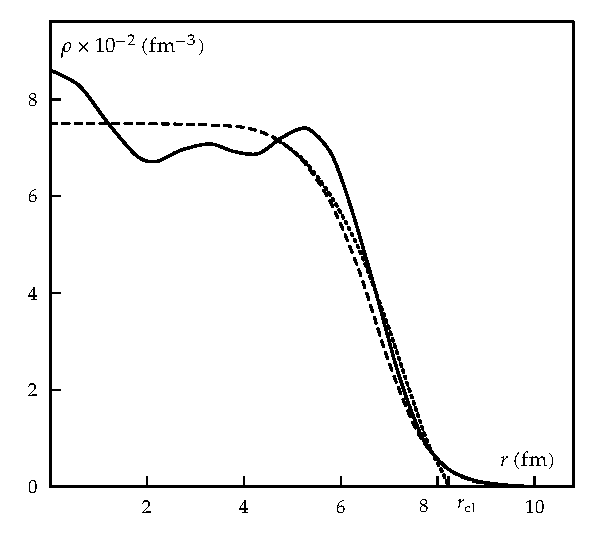
\includegraphics[width=0.75\textwidth]{pictures/13_1}
\par\end{centering}
\caption{\label{fig:13.1}图 13.1：在核子数$A=2N=184$的 Woods-Saxon 势阱中，精确密度（实线）与
Thomas-Fermi 近似（点线）的对比。势阱参数为：$V_{0}=-44\,\text{MeV}$，$a=0.67\,\text{fm}$，$R_{0}=1.27\,\text{fm}\cdot A^{1/3}$。虚线表示第
13.2.3 节的局域简谐近似（引自 \cite{DBS78}）。}
\end{figure}

总体而言，微观精确单粒子密度能够被式 (13.22) 这样简洁的形式描述到如此程度，是令人惊叹的。当我们利用式 (13.15) 结合
(13.19) 和 (13.6) 计算 Thomas-Fermi 近似下的基态总能量时，这一点表现得更加显著。采用与图 13.1 完全相同的势阱参数，数值积分计算结果为：

\[
E_{\mathrm{TF}}=-3194.5\,\text{MeV};\quad E_{\mathrm{exact}}=-3096.2\,\text{MeV}.
\]

在 Thomas-Fermi 近似下计算得到的重核结合能与精确微观值的相对偏差仅约为$\approx3\%$。这表明，在全空间积分的宏观大局物理量上，Thomas-Fermi
近似的精度甚至远高于单纯审视空间局域曲线（图 13.1）所能预期的水平。

比较式 (13.11) 与 (13.9)，可以直接得到如下微分恒等式：

\[
C^{\epsilon}(\boldsymbol{r},\boldsymbol{r}')=\partial_{\epsilon}\rho(\boldsymbol{r},\boldsymbol{r}';\epsilon),
\]

由此直接导出 Thomas-Fermi 近似下的能级态密度：

\[
g^{\mathrm{TF}}(\epsilon)=\frac{1}{2\pi^{2}}\left(\frac{2m}{\hbar^{2}}\right)^{3/2}\int\mathrm{d}^{3}r\,(\epsilon-V(\boldsymbol{r}))^{1/2}\Theta(\epsilon-V(\boldsymbol{r})).
\]

对于各向同性简谐振子势$V=\frac{1}{2}m\omega^{2}r^{2}$（我们在后文中将经常用它作为直观解析演示的标准范例），积分
(13.29) 可以完全解析积出，得到：

\[
g^{\mathrm{TF}}_{\mathrm{ho}}(\epsilon)=\frac{\epsilon^{2}}{2(\hbar\omega)^{3}}.
\]

在图 13.2 中，我们将该表达式对能量的积分（代表粒子数）与精确微观阶梯函数$N(\lambda)$进行了对比。我们再次看到，Thomas-Fermi
函数在宏观平均意义上极好地穿过了微观精确曲线\footnote{从$g^{\mathrm{TF}}(\epsilon)$在平均意义上代表精确态密度这一观察出发，我们无需使用极其繁复的“匹配连接条件”，即可立即直接导出通常的
WKB 量子化规则 \cite{Ar65}。关于 WKB 理论与 TF 理论如何系统联系的更详细内容，在此不作赘述 \cite{Vo77}。}；在后文中我们将对诸如$g(\epsilon)$等物理量的宏观“平均”如何严格数学定义给出更深入的讨论。

\begin{figure}[H]
\begin{centering}
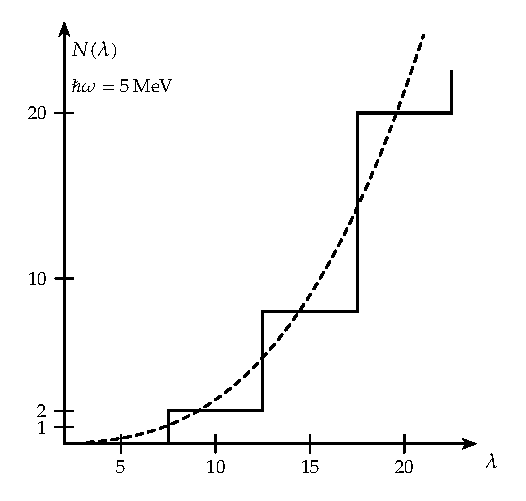
\includegraphics[width=0.65\textwidth]{pictures/13_2}
\par\end{centering}
\caption{\label{fig:13.2}图 13.2：简谐振子势中精确粒子数作为 Fermi 能的函数与相应 Thomas-Fermi 近似的对比。}
\end{figure}

为了计算 Thomas-Fermi 近似下的动能密度 (13.13)，我们结合式 (13.19) 和 (13.11)，得到：

\[
\tau^{\mathrm{TF}}(\boldsymbol{r})=\frac{1}{5\pi^{2}}\left(\frac{2m}{\hbar^{2}}\right)^{5/2}(\lambda-V(\boldsymbol{r}))^{5/2}\Theta(\lambda-V)=\frac{3}{5}\left(3\pi^{2}\right)^{2/3}\left(\rho^{\mathrm{TF}}\right)^{5/3}.
\]

在式 (13.31) 与 (13.22) 中消去$\lambda-V$，即建立起动能密度与局域密度之间的代数泛函关系（相应的式 (5.92)
计入了同位旋效应）：

\[
\tau^{\mathrm{TF}}=\frac{3}{5}(3\pi^{2})^{2/3}\rho^{5/3}.
\]

正如我们在引言中所指出的，由于两核子相互作用包含极强的短程性质，纯粹的 Thomas-Fermi 近似在核物理自洽场问题中几乎无能为力。这可以从以下事实清晰看出：对于
Skyrme 平均场势的局域部分$V[\rho]=a\rho+b\rho^{2}${[}参见式 (5.99){]}，非局域部分对它的修正极其微弱（这是核力短程性质的直接后果），式
(13.22) 关于密度$\rho$的解将导致空间各处完全均匀平庸的常数解，根本无法产生任何空间密度弥散分布。为了使半经典自洽理论在有限核中切实可行，我们必须对纯粹的
Thomas-Fermi 理论进行系统扩展，这将在随后的各小节中详尽讨论。

\subsection{Wigner-Kirkwood ℏ 展开\label{subsec:13.2.2_Wigner-Kirkwood=005C55=005F00}}

\subsubsection{形式体系\label{subsubsec:13.2.2.1_=005F62=005F0F=004F53=007CFB}}

我们现在希望展示，第 13.2.1 节中的 Thomas-Fermi 结果，实际上正是不同物理量（例如单粒子传播子 (13.2)）在按$\hbar$幂次作系统展开时的最低阶贡献。为此，转换至所谓的
Wigner 变换表象是极其方便的。单粒子算符$A$的 Wigner 变换定义为 \cite{Ar65}：

\[
A^{W}=A(\boldsymbol{q},\boldsymbol{p})=\int\mathrm{d}^{3}s\,e^{-\mathrm{i}\boldsymbol{p}\cdot\boldsymbol{s}/\hbar}\left\langle \boldsymbol{q}+\frac{1}{2}\boldsymbol{s}\right|A\left|\boldsymbol{q}-\frac{1}{2}\boldsymbol{s}\right\rangle ,
\]

其中$\boldsymbol{q}$与$\boldsymbol{s}$由式 (13.21) 给出。之所以采用 Wigner 表象极其便利，是因为在该表象中，例如
Hamiltonian (13.1) 恰好与其经典对应量严格一致：

\[
H^{W}(\boldsymbol{q},\boldsymbol{p})=\frac{\boldsymbol{p}^{2}}{2m}+V(\boldsymbol{q}).
\]

为了求出传播子 (13.2) 的完全经典部分，我们首先将其 Wigner 变换按$\beta$的幂次展开：

\[
C^{\beta}=e^{-\beta H}=\sum^{\infty}_{n=0}\frac{(-\beta)^{n}}{n!}H^{n}.
\]

这意味着我们必须求解单粒子算符乘积的 Wigner 变换。在附录 D 中，我们推导了如下乘积运算法则：

\[
(AB)^{W}=A(\boldsymbol{q},\boldsymbol{p})\exp\left[\frac{\mathrm{i}\hbar}{2}\left(\overleftarrow{\boldsymbol{\nabla}}_{\boldsymbol{q}}\cdot\overrightarrow{\boldsymbol{\nabla}}_{\boldsymbol{p}}-\overleftarrow{\boldsymbol{\nabla}}_{\boldsymbol{p}}\cdot\overrightarrow{\boldsymbol{\nabla}}_{\boldsymbol{q}}\right)\right]B(\boldsymbol{q},\boldsymbol{p}),
\]

其中箭头指示微分算符的作用方向：

\[
\Lambda=\frac{1}{2}\left(\overleftarrow{\boldsymbol{\nabla}}_{\boldsymbol{q}}\cdot\overrightarrow{\boldsymbol{\nabla}}_{\boldsymbol{p}}-\overleftarrow{\boldsymbol{\nabla}}_{\boldsymbol{p}}\cdot\overrightarrow{\boldsymbol{\nabla}}_{\boldsymbol{q}}\right).
\]

这一极其有用的式 (13.36) 使我们能够轻易验证诸如对易子的经典对应量正比于经典 Poisson 括号等著名结论 \cite{Go59}。利用式
(13.36)，我们亦可逐阶计算出展开 (13.35) 中出现的各阶项。例如计算至二阶项：

\[
(H^{2})^{W}=(H^{W})^{2}-\frac{\hbar^{2}}{4m}\Delta V.
\]

式 (13.38) 中的$\hbar$修正项源自动量算符与势能算符的非对易性。单粒子传播子 (13.2) 中正是源于动能部分与势能部分不对易而产生的这种$\hbar$依赖性，构成了我们所关注的焦点，也是我们旨在按$\hbar$的幂级数进行系统展开的对象；因此，在
Wigner 表象下我们无需担忧隐藏在$\beta$或其他表象转换过程中可能产生的其他微观依赖性。根据上述讨论显然可以看出，我们所讨论的$\hbar$展开借助展开式
(13.35) 与乘积法则 (13.36) 变得完全可行；$\hbar$的幂次在非经典修正项中始终为偶数，且精确等于特定项中关于空间与动量导数的阶数之和。因此，该展开在本质上同时也是一种梯度展开（gradient
expansion）。按$\hbar$的最低阶（零阶）表达式由 (13.35)、(13.36) 和 (13.38) 易于算出：

\[
C^{\beta}_{0}(\boldsymbol{q},\boldsymbol{p})=\exp\left[-\beta\left(\frac{p^{2}}{2m}+V(\boldsymbol{q})\right)\right].
\]

计算其逆 Wigner 变换，即对动量执行 Fourier 变换，恰好给出了我们之前在式 (13.19) 中得到的传播子局域 Thomas-Fermi
近似表达式。我们看到，Wigner 表象下的零阶项直接就是经典统计算符。由于式 (13.35) 是按$\hbar$与$\beta$的联立展开，对于高温（即极小的$\beta$），我们自然回归到经典统计物理结果。必须再次强调，在我们的核物理背景中，$\beta$绝不代表倒温度；相反，我们研究的是处于零温$T=0$的
Fermi 简并体系。另一方面，极其重要的一点在于：Thomas-Fermi 近似及其在随后的推导中所建立的扩展形式，严格遵循 Pauli
不相容原理。通过结合 (13.39) 与 (13.11) 从其 Wigner 变换直接计算密度，可以最为清晰地看出这一点：

\[
\rho^{\mathrm{TF}}(\boldsymbol{q})=\frac{2}{(2\pi\hbar)^{3}}\int\mathrm{d}^{3}p\,\mathcal{L}^{-1}_{\beta\to\lambda}\left[\frac{C^{\beta}_{0}(\boldsymbol{q},\boldsymbol{p})}{\beta}\right]=\frac{2}{(2\pi\hbar)^{3}}\int\mathrm{d}^{3}p\,\Theta\left(\lambda-\frac{p^{2}}{2m}-V(\boldsymbol{q})\right),
\]

\[
=\frac{1}{3\pi^{2}\hbar^{3}}[2m(\lambda-V(\boldsymbol{q}))]^{3/2}\Theta(\lambda-V(\boldsymbol{q})),
\]

这无非是对从零直至 Fermi 能级的所有有效量子动量$p\le[2m(\lambda-V)]^{1/2}$的相空间状态求和，且每个能级被自旋向上与向下的两个核子完全占据。

式 (13.35) 中$\beta$的幂次与$\hbar$的幂次并不是简单同步的，为了精确保留至$\hbar^{2}$阶，我们必须将式
(13.35) 展开至$\beta^{3}$阶。严格计算的结果为 \cite{Wi32,Wi34,Ki33,Ki57,JB75}：

\[
C^{\beta}(\boldsymbol{q},\boldsymbol{p})=\exp\left[-\beta\left(\frac{p^{2}}{2m}+V(\boldsymbol{q})\right)\right]\left\{ 1+\hbar^{2}\left[-\frac{\beta^{2}}{8m}\Delta V+\frac{\beta^{3}}{24m}(\boldsymbol{\nabla}V)^{2}+\frac{\beta^{3}}{24m^{2}}(\boldsymbol{p}\cdot\boldsymbol{\nabla})^{2}V\right]+\mathcal{O}(\hbar^{4})\right\} .
\]

表达式 (13.42) 使我们能够对第 13.2.1 节所考察的全部物理量获得系统的半经典量子修正。结合式 (13.11)，例如对于半经典密度矩阵的
Wigner 变换$f_{\mathrm{sc}}$（关于包含自旋-轨道耦合项的系统推广，参见 \cite{JBB75}），我们得到：

\[
f_{\mathrm{sc}}(\boldsymbol{q},\boldsymbol{p};\lambda)=\Theta\left(\lambda-\frac{p^{2}}{2m}-V(\boldsymbol{q})\right)+\hbar^{2}\left\{ -\frac{1}{8m}\Delta V\,\delta'\left(\lambda-\frac{p^{2}}{2m}-V\right)+\left[\frac{1}{24m}(\boldsymbol{\nabla}V)^{2}+\frac{1}{24m^{2}}(\boldsymbol{p}\cdot\boldsymbol{\nabla})^{2}V\right]\delta''\left(\lambda-\frac{p^{2}}{2m}-V\right)\right\} +\mathcal{O}(\hbar^{4}),
\]

式中半经典化学势$\lambda_{\mathrm{sc}}$由粒子数归一化约束 (13.14) 决定。在式 (13.43) 中，我们暂且忽略了正幂次$\beta$的逆
Laplace 变换在严格数学意义上不存在的问题。形式上通过将式 (13.11) 对$\lambda$进行微商来产生式 (13.42)
中不同幂次的$\beta$，我们在式 (13.43) 中获得了关于$\delta$函数的各阶导数。表达式 (13.43) 显然只能在广义函数（分布）的意义下加以理解与使用，但我们必须更深入地考察传播子的半经典展开
(13.42) 究竟在何种物理途径下才能发挥其强大威力。对动量$\boldsymbol{p}$积分式 (13.43)，我们直接获得包含二级梯度修正的半经典粒子数密度：

\[
\rho_{\mathrm{sc}}(\boldsymbol{r})=\frac{1}{3\pi^{2}}\left(\frac{2m}{\hbar^{2}}\right)^{3/2}(\lambda_{\mathrm{sc}}-V(\boldsymbol{r}))^{3/2}-\frac{1}{24\pi^{2}}\left(\frac{2m}{\hbar^{2}}\right)^{1/2}\left[\frac{\Delta V}{(\lambda_{\mathrm{sc}}-V)^{1/2}}+\frac{1}{4}\frac{(\boldsymbol{\nabla}V)^{2}}{(\lambda_{\mathrm{sc}}-V)^{3/2}}\right].
\]

这一半经典密度表达式不再包含任何阶跃$\delta$函数，然而在经典转折点$\lambda_{\mathrm{sc}}-V=0$处它发生病态发散，这使得我们必须重新审视此类展开的物理意义与适用范围。

\subsubsection{ℏ 展开的适用性与解释\label{subsubsec:13.2.2.2_=009002=007528=006027=004E0E=0089E3=0091CA}}

为了研究展开式 (13.42) 与 (13.43) 的有效性，考察若干能够严格解析求出传播子的理想势阱范例是极具启发性的：

(i) 对于一维线性势$V_{1}=ax$，容易验证如下传播子形式严格满足 Schrödinger 方程 (13.3)：

\[
C_{1}(x,x')=C^{(0)}_{1}(x,x')\exp\left[\frac{\hbar^{2}\beta^{3}}{24m}(V'_{1})^{2}\right],
\]

式中$V'_{1}$表示势场的一阶导数，而$C^{(0)}_{1}(x,x')$则是单粒子传播子 Thomas-Fermi 近似
(13.19) 的一维对应形式。式 (13.45) 的 Wigner 变换仅作用于$C^{(0)}_{1}$，剩余指数因子的半经典展开与式
(13.42) 括号中的表达式完全吻合；这可以轻而易举地加以验证。由此亦极其清楚地表明，对于此范例，展开 (13.42) 是完全严格成立的，并且在整个复$\beta$与$\hbar$平面上一致收敛。然而，在计算物理可观测量
{[}参见式 (13.7)–(13.15){]} 时，我们必须对形如 (13.42) 的展开执行逆 Laplace 变换，由此便产生了与式
(13.43) 相关联的数学困难。针对线性势范例 (13.45)，我们可以进行更详细的考察。利用式 (13.40) 以及 Laplace
变换的卷积定理 \cite{PB55,AS65}，线性势下的密度可以严格积出：

\[
f_{1}(q,p;\lambda)=2^{2/3}\sigma\int^{\infty}_{0}\mathrm{d}E\,\Theta\left(\lambda-\frac{p^{2}}{2m}-V_{1}(q)-E\right)\mathrm{Ai}\left(-2^{2/3}\sigma E\right),
\]

其中特征参数与 Airy 函数的积分表示分别为 \cite{AS65}：

\[
\sigma=\left(\frac{2m}{\hbar^{2}(V'_{1})^{2}}\right)^{1/3},\quad\mathrm{Ai}(z)=\frac{1}{2\pi}\int^{\infty}_{-\infty}\mathrm{d}s\,e^{\mathrm{i}(s^{3}/3+zs)}.
\]

在式 (13.47) 中作变量代换$y=2^{2/3}\sigma\beta$，我们看到当$\hbar\to0$时，$\mathrm{Ai}$渐近正比于$\delta(E)$，从而结合式
(13.46) 立即重新恢复出式 (13.43) 的首批主要项。通过将式 (13.45) 展开至$\hbar^{2}$，更高阶修正项亦可完全重现。由此我们可以洞察所有数学佯谬的根源：式
(13.46) 在本质上关于$\hbar$是非解析的，因此严格的常规$\hbar$幂级数展开在局域层面并不存在（这与函数$e^{-a/x}$在原点关于$x$的本性奇点完全类似）。

(ii) 作为第二个确定的解析范例，我们考察三维各向同性简谐振子势$V_{2}=\frac{1}{2}m\omega^{2}r^{2}$。容易验证，相应的含时
Schrödinger 方程 (13.3) 具有如下精确传播子解（详细推导可参见 \cite{Kr64}）：

\[
C_{2}(\boldsymbol{r},\boldsymbol{r}';\beta)=\left(\frac{m\omega}{2\pi\hbar\sinh(\beta\hbar\omega)}\right)^{3/2}\exp\left\{ -\frac{m\omega}{2\hbar\sinh(\beta\hbar\omega)}\left[(\boldsymbol{r}^{2}+\boldsymbol{r}'^{2})\cosh(\beta\hbar\omega)-2\boldsymbol{r}\cdot\boldsymbol{r}'\right]\right\} .
\]

在式 (13.15) 中我们需要该传播子的迹，容易算出其解析结果为：

\[
Z_{2}(\beta)=\mathrm{Tr}\,C^{\beta}_{2}=\frac{1}{4\sinh^{3}(\beta\hbar\omega/2)}.
\]

为了计算有效结合能项$E-\lambda N$，我们需要求出$\beta^{-2}Z(\beta)$的逆 Laplace 变换。对于式
(13.49) 的配分函数$Z_{2}$，这可以通过在复平面上沿虚轴左侧闭合围道积分来完成（取$\lambda>0$）。围道积分包含来自配分函数$Z_{2}$沿虚轴上每一个极点的留数贡献。原点$\beta=0$处的极点为五阶极点，而虚轴上的其他极点仅为三阶极点。为了计算原点处的留数，我们只需写出$Z_{2}(\beta)\beta^{-2}$直至$\beta^{-1}$阶的
Laurent 级数展开：

\[
\frac{Z_{2}(\beta)}{\beta^{2}}=\frac{2}{(\hbar\omega)^{3}}\frac{1}{\beta^{5}}\left[1-\frac{1}{8}(\beta\hbar\omega)^{2}+\frac{17}{1920}(\beta\hbar\omega)^{4}+\dots\right].
\]

计入原点极点以及虚轴上所有其余振荡极点的留数，我们获得能量的完整解析表达式：

\[
E-\lambda N=-\frac{\lambda^{4}}{12(\hbar\omega)^{3}}+\frac{\lambda^{2}}{8\hbar\omega}-\frac{17\hbar\omega}{960}+\dots+\text{（振荡项）}.
\]

从式 (13.51) 可以看出极其优美的物理图像：来自复原点$\beta=0$极点的贡献，作为$\lambda$的函数给出了一个单调平滑增长的部分；而远离实轴、沿虚轴分布的所有其余极点，则贡献出周期性剧烈振荡的项。这些振荡显然正是源于三维简谐势中高度简并的分立能级结构，而在单调线性势
(13.45) 中完全不存在这类虚轴极点。

尽管简谐振子势是非常特殊的解析范例，但我们完全可以将其核心物理结论推广至任意一般势阱：在式 (13.15) 中，函数$e^{\beta\lambda}Z(\beta)\beta^{-2}$在复原点处的奇点贡献直接给出了基态结合能的平滑宏观部分（液滴能），而分布在复平面其余位置的所有非零奇点贡献则直接构成了壳效应量子振荡项。

为了进一步证实这一点，我们考察第 2.9 节中研究的 Strutinsky 能级平滑方法与上述原点留数展开之间的严格数学联系。考察经曲率修正的高斯平滑态密度
(2.109)：

\[
\tilde{g}(\epsilon)=\frac{1}{\gamma}\int^{\infty}_{-\infty}\mathrm{d}\epsilon'\,g(\epsilon')f_{M}\left(\frac{\epsilon-\epsilon'}{\gamma}\right).
\]

利用配分函数的 Laplace 变换定义及卷积定理，对应于平滑态密度的平滑配分函数为：

\[
\tilde{Z}_{M}(\beta)=Z(\beta)\tilde{f}_{M}(\beta\gamma),
\]

其中平滑因子的 Laplace 变换为：

\[
\tilde{f}_{M}(\beta\gamma)=w(\beta\gamma)\sum^{M}_{m=0}\frac{(-1)^{m}}{2^{2m}m!}H_{2m}(0)(\beta\gamma)^{2m},
\]

\[
w(\beta\gamma)=e^{\beta^{2}\gamma^{2}/4}.
\]

在第 2.9 节中我们证明了，Strutinsky 平滑参数$\gamma$的取值必须在主壳间距$\hbar\omega$或更大的量级。这导致式
(13.54) 中的因子在振子配分函数 (13.49) 的第一个虚轴奇点处衰减了整整五个数量级以上！换言之，Strutinsky 平滑过程在物理本质上等价于在正负虚轴奇点之间截取一段配分函数，它尽可能长时间地保持等于精确配分函数，并在靠近壳层极点时以宽度$\gamma$迅速平滑降为零。因此，Strutinsky
平滑程序与我们上述将平滑能量定义为式 (13.15) 中来自$Z(\beta)$在原点处小$\beta$渐近行为的贡献是完全等价的
\cite{Je73,Je76}。

因此，式 (13.42) 所给出的半经典展开的巨大实用价值正在于：它直接提供了配分函数在原点附近关于$\hbar$与$\beta$的联立
Laurent 级数；这正是我们在计算来自原点奇点的结合能贡献时所需的全部物理信息。\footnote{应当指出，通过利用 Laurent 级数构建相应的 Padé 近似，原则上可以从$Z(\beta)$的半经典展开 (13.50)
重建其极点结构，从而将部分振荡壳效应重新包含进结合能中。然而，这一方向迄今尚未得到非常深入的系统研究 \cite{GS77}。}

\begin{table}[H]
\caption{\label{tab:13.1}表 13.1：与图 13.1 相同参数的球形 Woods-Saxon 势阱中的平滑结合能量（单位均为
MeV）。第一列为核子数$A=2N=2Z$。第二、三、四列分别给出$E_{\mathrm{TF}}$、$E^{(2)}_{\mathrm{sc}}$和$E^{(4)}_{\mathrm{sc}}$，分别对应式
(13.42) 中 TF 项、$\mathcal{O}(\hbar^{2})$项及$\mathcal{O}(\hbar^{4})$项的贡献。第五列给出总半经典能量$E_{\mathrm{sc}}$，最后一列给出
Strutinsky 平滑能量（引自 \cite{Je76}）。}

\centering{}<lyxtabular version=\textquotedbl 3\textquotedbl{} rows=\textquotedbl 4\textquotedbl{}
columns=\textquotedbl 6\textquotedbl ><features rotate=\textquotedbl 0\textquotedbl{}
tabularvalignment=\textquotedbl middle\textquotedbl ><column alignment=\textquotedbl center\textquotedbl{}
valignment=\textquotedbl top\textquotedbl ><column alignment=\textquotedbl center\textquotedbl{}
valignment=\textquotedbl top\textquotedbl ><column alignment=\textquotedbl center\textquotedbl{}
valignment=\textquotedbl top\textquotedbl ><column alignment=\textquotedbl center\textquotedbl{}
valignment=\textquotedbl top\textquotedbl ><column alignment=\textquotedbl center\textquotedbl{}
valignment=\textquotedbl top\textquotedbl ><column alignment=\textquotedbl center\textquotedbl{}
valignment=\textquotedbl top\textquotedbl ><row><cell alignment=\textquotedbl center\textquotedbl{}
valignment=\textquotedbl top\textquotedbl{} topline=\textquotedbl true\textquotedbl{}
bottomline=\textquotedbl true\textquotedbl{} leftline=\textquotedbl true\textquotedbl{}
usebox=\textquotedbl none\textquotedbl >$A$</cell><cell alignment=\textquotedbl center\textquotedbl{}
valignment=\textquotedbl top\textquotedbl{} topline=\textquotedbl true\textquotedbl{}
bottomline=\textquotedbl true\textquotedbl{} leftline=\textquotedbl true\textquotedbl{}
usebox=\textquotedbl none\textquotedbl >$E_{\mathrm{TF}}$</cell><cell
alignment=\textquotedbl center\textquotedbl{} valignment=\textquotedbl top\textquotedbl{}
topline=\textquotedbl true\textquotedbl{} bottomline=\textquotedbl true\textquotedbl{}
leftline=\textquotedbl true\textquotedbl{} usebox=\textquotedbl none\textquotedbl >$E^{(2)}_{\mathrm{sc}}$</cell><cell
alignment=\textquotedbl center\textquotedbl{} valignment=\textquotedbl top\textquotedbl{}
topline=\textquotedbl true\textquotedbl{} bottomline=\textquotedbl true\textquotedbl{}
leftline=\textquotedbl true\textquotedbl{} usebox=\textquotedbl none\textquotedbl >$E^{(4)}_{\mathrm{sc}}$</cell><cell
alignment=\textquotedbl center\textquotedbl{} valignment=\textquotedbl top\textquotedbl{}
topline=\textquotedbl true\textquotedbl{} bottomline=\textquotedbl true\textquotedbl{}
leftline=\textquotedbl true\textquotedbl{} usebox=\textquotedbl none\textquotedbl >$E_{\mathrm{sc}}$</cell><cell
alignment=\textquotedbl center\textquotedbl{} valignment=\textquotedbl top\textquotedbl{}
topline=\textquotedbl true\textquotedbl{} bottomline=\textquotedbl true\textquotedbl{}
leftline=\textquotedbl true\textquotedbl{} rightline=\textquotedbl true\textquotedbl{}
usebox=\textquotedbl none\textquotedbl >$E_{\mathrm{Str}}$</cell></row><row><cell
alignment=\textquotedbl center\textquotedbl{} valignment=\textquotedbl top\textquotedbl{}
topline=\textquotedbl true\textquotedbl{} leftline=\textquotedbl true\textquotedbl{}
usebox=\textquotedbl none\textquotedbl >164</cell><cell alignment=\textquotedbl center\textquotedbl{}
valignment=\textquotedbl top\textquotedbl{} topline=\textquotedbl true\textquotedbl{}
leftline=\textquotedbl true\textquotedbl{} usebox=\textquotedbl none\textquotedbl >-3344.7</cell><cell
alignment=\textquotedbl center\textquotedbl{} valignment=\textquotedbl top\textquotedbl{}
topline=\textquotedbl true\textquotedbl{} leftline=\textquotedbl true\textquotedbl{}
usebox=\textquotedbl none\textquotedbl >88.8</cell><cell alignment=\textquotedbl center\textquotedbl{}
valignment=\textquotedbl top\textquotedbl{} topline=\textquotedbl true\textquotedbl{}
leftline=\textquotedbl true\textquotedbl{} usebox=\textquotedbl none\textquotedbl >1.0</cell><cell
alignment=\textquotedbl center\textquotedbl{} valignment=\textquotedbl top\textquotedbl{}
topline=\textquotedbl true\textquotedbl{} leftline=\textquotedbl true\textquotedbl{}
usebox=\textquotedbl none\textquotedbl >-3254.9</cell><cell alignment=\textquotedbl center\textquotedbl{}
valignment=\textquotedbl top\textquotedbl{} topline=\textquotedbl true\textquotedbl{}
leftline=\textquotedbl true\textquotedbl{} rightline=\textquotedbl true\textquotedbl{}
usebox=\textquotedbl none\textquotedbl >-3256.0 (1.2)</cell></row><row><cell
alignment=\textquotedbl center\textquotedbl{} valignment=\textquotedbl top\textquotedbl{}
topline=\textquotedbl true\textquotedbl{} leftline=\textquotedbl true\textquotedbl{}
usebox=\textquotedbl none\textquotedbl >260</cell><cell alignment=\textquotedbl center\textquotedbl{}
valignment=\textquotedbl top\textquotedbl{} topline=\textquotedbl true\textquotedbl{}
leftline=\textquotedbl true\textquotedbl{} usebox=\textquotedbl none\textquotedbl >-5484.8</cell><cell
alignment=\textquotedbl center\textquotedbl{} valignment=\textquotedbl top\textquotedbl{}
topline=\textquotedbl true\textquotedbl{} leftline=\textquotedbl true\textquotedbl{}
usebox=\textquotedbl none\textquotedbl >119.7</cell><cell alignment=\textquotedbl center\textquotedbl{}
valignment=\textquotedbl top\textquotedbl{} topline=\textquotedbl true\textquotedbl{}
leftline=\textquotedbl true\textquotedbl{} usebox=\textquotedbl none\textquotedbl >1.1</cell><cell
alignment=\textquotedbl center\textquotedbl{} valignment=\textquotedbl top\textquotedbl{}
topline=\textquotedbl true\textquotedbl{} leftline=\textquotedbl true\textquotedbl{}
usebox=\textquotedbl none\textquotedbl >-5364.0</cell><cell alignment=\textquotedbl center\textquotedbl{}
valignment=\textquotedbl top\textquotedbl{} topline=\textquotedbl true\textquotedbl{}
leftline=\textquotedbl true\textquotedbl{} rightline=\textquotedbl true\textquotedbl{}
usebox=\textquotedbl none\textquotedbl >-5364.4 (0.8)</cell></row><row><cell
alignment=\textquotedbl center\textquotedbl{} valignment=\textquotedbl top\textquotedbl{}
topline=\textquotedbl true\textquotedbl{} bottomline=\textquotedbl true\textquotedbl{}
leftline=\textquotedbl true\textquotedbl{} usebox=\textquotedbl none\textquotedbl >416</cell><cell
alignment=\textquotedbl center\textquotedbl{} valignment=\textquotedbl top\textquotedbl{}
topline=\textquotedbl true\textquotedbl{} bottomline=\textquotedbl true\textquotedbl{}
leftline=\textquotedbl true\textquotedbl{} usebox=\textquotedbl none\textquotedbl >-9049.1</cell><cell
alignment=\textquotedbl center\textquotedbl{} valignment=\textquotedbl top\textquotedbl{}
topline=\textquotedbl true\textquotedbl{} bottomline=\textquotedbl true\textquotedbl{}
leftline=\textquotedbl true\textquotedbl{} usebox=\textquotedbl none\textquotedbl >162.5</cell><cell
alignment=\textquotedbl center\textquotedbl{} valignment=\textquotedbl top\textquotedbl{}
topline=\textquotedbl true\textquotedbl{} bottomline=\textquotedbl true\textquotedbl{}
leftline=\textquotedbl true\textquotedbl{} usebox=\textquotedbl none\textquotedbl >1.1</cell><cell
alignment=\textquotedbl center\textquotedbl{} valignment=\textquotedbl top\textquotedbl{}
topline=\textquotedbl true\textquotedbl{} bottomline=\textquotedbl true\textquotedbl{}
leftline=\textquotedbl true\textquotedbl{} usebox=\textquotedbl none\textquotedbl >-8881.5</cell><cell
alignment=\textquotedbl center\textquotedbl{} valignment=\textquotedbl top\textquotedbl{}
topline=\textquotedbl true\textquotedbl{} bottomline=\textquotedbl true\textquotedbl{}
leftline=\textquotedbl true\textquotedbl{} rightline=\textquotedbl true\textquotedbl{}
usebox=\textquotedbl none\textquotedbl >-8882.8 (1.2)</cell></row></lyxtabular>
\end{table}

在表 13.1 中，我们展示了球形 Woods-Saxon 势阱中基态能量平滑部分的逐阶收敛情况，并与精确的 Strutinsky
平滑值进行了严格比对。极为引人注目的是：包含至$\hbar^{4}$阶展开即可获得高度精确收敛的宏观数值，且与 Strutinsky
能量在极高精度下完美吻合。来自复原点极点的半经典能量几乎穷尽了体系基态总能量的绝大部分（微观壳效应仅占千分之几的量级）。然而，这千分之几的细微能量起伏包含了原子核形变势能面上诸如双裂变势垒等极具决定性的微观结构效应。

\subsubsection{动能密度泛函\label{subsubsec:13.2.2.3_=0052A8=0080FD=005BC6=005EA6=006CDB=0051FD}}

克服无法直接开展自洽半经典迭代计算困难的一个极具吸引力的突破口如下\footnote{在本节的讨论中，我们在很大程度上参考了 \cite{Bs77} 中给出的阐述。}：在计算基态能量时，我们需要式
(13.13) 所定义的动能密度$\tau(\boldsymbol{r})$。如果我们能够将动能密度完全表达为局域密度$\rho(\boldsymbol{r})$的泛函，即$\tau=\tau[\rho(\boldsymbol{r})]$，那么由于诸如
Skyrme 势能密度 (5.87) 本身完全由$\rho$和$\tau$构成，原子核总结合能将成为局域密度$\rho(\boldsymbol{r})$的纯粹单变量泛函。随后只需对$\rho$进行能量变分，即可直接导出关于局域密度$\rho(\boldsymbol{r})$的闭合微分方程。尽管
Hohenberg-Kohn 定理 \cite{HK64,MT77} 已经从理论上严格确立了任意多 Fermion 体系的基态能量及动能密度都是局域密度的唯一泛函，但在实际微观计算中推导这一泛函的精确解析形式是极端困难的。而在我们的半经典理论体系中，我们却能够系统构造出完全自洽的渐近泛函形式：

\[
\tau_{\mathrm{sc}}(\boldsymbol{r},\lambda)=\frac{3}{5}\left(\frac{2m}{\hbar^{2}}\right)^{5/2}\frac{1}{3\pi^{2}}(\lambda-V)^{5/2}-\frac{\hbar^{2}}{8m}\frac{1}{3\pi^{2}}\left(\frac{2m}{\hbar^{2}}\right)^{3/2}\left[5\Delta V(\lambda-V)^{1/2}-\frac{9}{4}\frac{(\boldsymbol{\nabla}V)^{2}}{(\lambda-V)^{1/2}}\right]+\mathcal{O}(\hbar^{4}).
\]

将密度表达式 (13.44) 及其梯度展开结合，消去势场导数，最终导出了著名的动能密度泛函 \cite{Ki67,Je76}\footnote{有时为了更精确地重现表面能，人们会采用略微不同于$1/36$的唯象唯理加权系数 \cite{Ba72b}。}：

\[
\tau[\rho]=\frac{3}{5}(3\pi^{2})^{2/3}\rho^{5/3}+\frac{1}{36}\frac{(\boldsymbol{\nabla}\rho)^{2}}{\rho}+\frac{1}{3}\Delta\rho.
\]

式 (13.57) 右端第一项正是无限均匀核物质的 Thomas-Fermi 主导项；第二项被称为 Weizsäcker 梯度修正项；而最后一项为空间全散度项，由
Gauss 定理可知它对全空间动能积分不产生净贡献。

\begin{figure}[H]
\begin{centering}
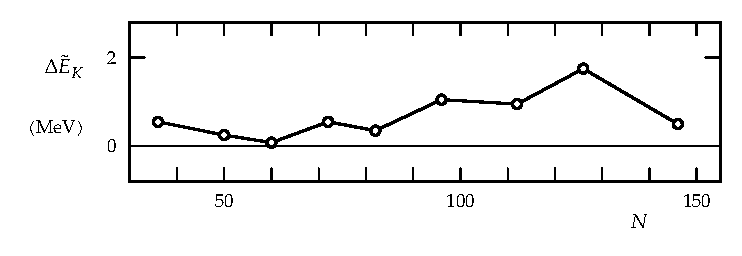
\includegraphics[width=0.65\textwidth]{pictures/13_3}
\par\end{centering}
\caption{\label{fig:13.3}图 13.3：动能差值$\Delta\tilde{E}_{K}=\tilde{E}_{K}-\tilde{T}_{K}$，其中$\tilde{E}_{K}$为
Strutinsky 平滑动能，$\tilde{T}_{K}$按文中动能泛函计算。数值为球形 Woods-Saxon 势阱中作为中子数$N$的函数（引自
\cite{BJC76}）。}
\end{figure}


\subsubsection{变分计算\label{subsubsec:13.2.2.4_=0053D8=005206=008BA1=007B97}}

获得泛函 (13.57) 后，我们即可通过变分原理自洽确定半经典密度分布\footnote{此处的变分原理在与一般能量泛函$E[\rho]$相联系时，并不严格等同于第 5.6.1.2 节中基于多体态矢的 Ritz 严格上界变分。}：

\[
\delta\left(E[\rho]-\lambda\int\mathrm{d}^{3}r\,\rho(\boldsymbol{r})\right)=0.
\]

为展示核心物理图像，忽略有效质量与自旋-轨道耦合项，取能量密度泛函为：

\[
E[\rho]=\int\mathrm{d}^{3}r\,\mathcal{E}[\rho],\quad\mathcal{E}[\rho]=\mathcal{E}_{\infty}(\rho)+\frac{\hbar^{2}}{2m}\frac{1}{36}\frac{(\boldsymbol{\nabla}\rho)^{2}}{\rho},
\]

在核物质饱和密度$\rho_{0}\approx0.14\,\text{fm}^{-3}$附近将其参数化展开为不可压缩模量$K$的形式：

\[
\mathcal{E}_{\infty}(\rho)\simeq\mathcal{E}_{0}+\frac{K}{18}\left(\frac{\rho-\rho_{0}}{\rho_{0}}\right)^{2}.
\]

变分方程直接导出密度的二阶非线性常微分方程：

\[
\Delta\rho-\frac{1}{2}\frac{(\boldsymbol{\nabla}\rho)^{2}}{\rho}-\frac{18m}{\hbar^{2}}\rho\frac{\partial\mathcal{E}_{\infty}}{\partial\rho}+\frac{18m}{\hbar^{2}}\lambda\rho=0.
\]

在核表面渐近区，式 (13.62) 简化为 Berg-Wilets 方程 \cite{BW56}：

\[
\Delta\sqrt{\rho}-\frac{1}{a^{2}}\sqrt{\rho}=0,
\]

其球对称渐近解具有指数衰减形式：

\[
\rho(r)\sim\frac{1}{r^{2}}e^{-2r/a}.
\]

\begin{figure}[H]
\begin{centering}
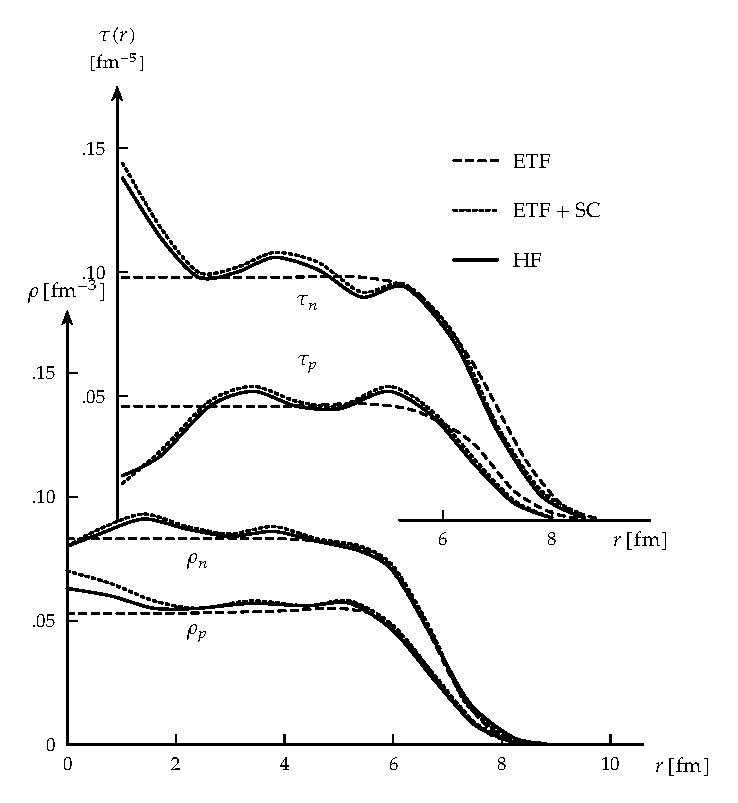
\includegraphics[width=0.75\textwidth]{pictures/13_4}
\par\end{centering}
\caption{\label{fig:13.4}图 13.4：自洽半经典密度与动能密度剖面与 Skyrme Hartree-Fock 微观精确结果的对比
\cite{BCK76}。}
\end{figure}


\subsection{ℏ 展开的部分求和\label{subsec:13.2.3_=0090E8=005206=006C42=00548C}}

上一小节表明，虽然扩展 Thomas-Fermi 能够极好地给出能量的平滑部分，但在经典转折点附近其密度仍显现出过陡的下降行为。为了解决这一局限，我们重新审视展开
(13.16)。如果在一维情形下保留一阶导数（线性化势场），传播子严格解析可求 \cite{Sw55,Gr72,DBS78}：

\[
C^{(1)}(q,s)=\left(\frac{m}{2\pi\hbar^{2}\beta}\right)^{1/2}\exp\left[-\frac{m}{2\hbar^{2}\beta}s^{2}-\beta V(q)+\frac{\hbar^{2}\beta^{3}}{24m}\left(\frac{\partial V}{\partial q}\right)^{2}\right].
\]

进一步在展开 (13.16) 中保留至势场的二阶导数项，即构建所谓的局域简谐近似（locally harmonic approximation）。借助简谐振子解
(13.48) 作为指导，一维局域简谐传播子的严格解析表达式为 \cite{Gr72,DBS78}：

\[
C^{(2)}(q,s)=\left(\frac{m\omega(q)}{2\pi\hbar\sinh(\beta\hbar\omega(q))}\right)^{1/2}\exp\left\{ -\frac{m\omega(q)}{4\hbar}\left[\tanh\left(\frac{\beta\hbar\omega(q)}{2}\right)s^{2}+4\frac{(q-\bar{q})^{2}}{\tanh\left(\frac{\beta\hbar\omega(q)}{2}\right)}\right]-\beta\bar{V}(q)\right\} ,
\]

其中特征参数定义为：$\omega(q)=[V''(q)/m]^{1/2}$，$\bar{q}(q)=q-V'(q)/V''(q)$，以及$\bar{V}(q)=V(q)-[V'(q)]^{2}/[2V''(q)]$。这一部分求和方案极其出色地再现了波函数向经典禁区穿透的量子隧道效应。

\begin{figure}[H]
\begin{centering}
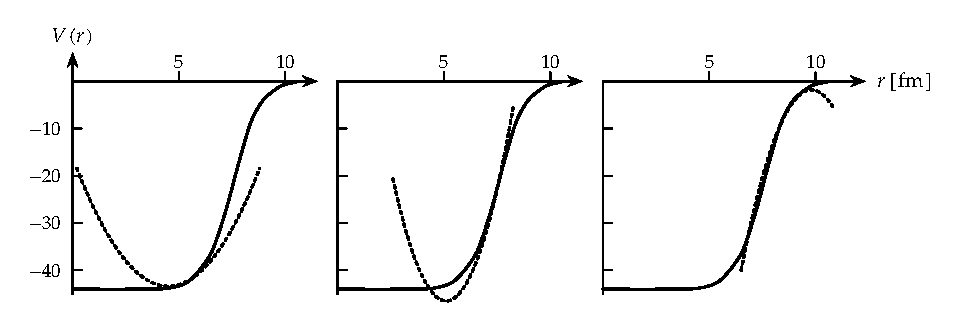
\includegraphics[width=0.65\textwidth]{pictures/13_5}
\par\end{centering}
\caption{\label{fig:13.5}图 13.5：在一维 Woods-Saxon 势阱中三个不同坐标点处的局域抛物线近似。}
\end{figure}


\subsection{鞍点法\label{subsec:13.2.4_=00978D=0070B9=006CD5}}

为了从局域简谐传播子中解析抽取平滑态密度与能量，可以高效借助复平面鞍点法（Saddle Point Method, SPM）\cite{PB75,Bh77}。将逆
Laplace 积分写为$G(\lambda)=\frac{1}{2\pi\mathrm{i}}\int^{c+\mathrm{i}\infty}_{c-\mathrm{i}\infty}\mathrm{d}\beta\,e^{S(\beta)}$，并将指数项$S$在实轴驻点$\beta_{0}$处展开，系统考虑高阶涨落修正。

\begin{figure}[H]
\begin{centering}
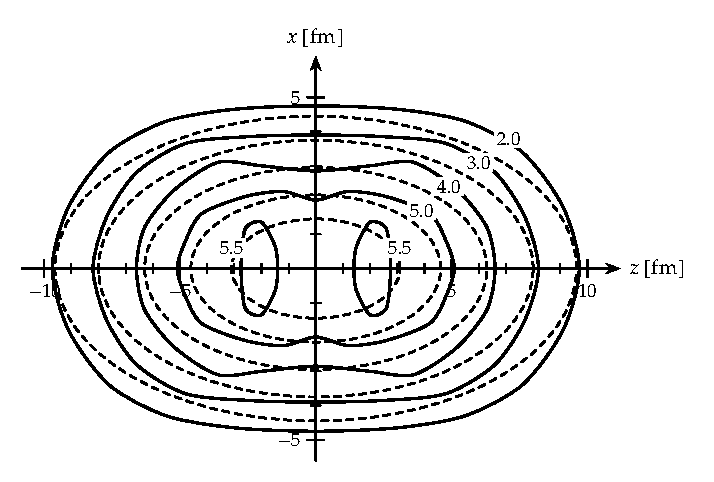
\includegraphics[width=0.75\textwidth]{pictures/13_6}
\par\end{centering}
\caption{\label{fig:13.6}图 13.6：强形变简谐振子势中，微观精确密度与采用鞍点法获得的平滑半经典密度的对比（感谢 J.
Bartel 提供此图）。}
\end{figure}


\subsection{球形 Woods-Saxon 势的应用\label{subsec:13.2.5_Woods-Saxon=005E94=007528}}

结合局域简谐传播子 (13.66) 与鞍点法，构成了本理论的核心基础。在图 13.1 中，采用局域简谐近似获得的密度（虚线）在核表面弥散尾区与精确微观结果展现出令人信服的极佳吻合，彻底克服了原
ETF 密度泛函在表面过渡过陡的理论缺陷。平均单粒子能量和与 Strutinsky 宏观平滑值在全质量区内的偏差仅在 5–10 MeV
范围以内。

\subsection{对性质的半经典处理\label{subsec:13.2.6_=005BF9=006027=008D28=005904=007406}}

在建立起自洽单粒子密度的半经典描述后，将其推广至包含配对关联的 BCS 理论框架是非常自然的（参见第 6、7 章）。在极限$\hbar\to0$下，广义准粒子密度对易子方程退化为经典
Poisson 括号，由此直接导出半经典能隙方程（gap equation）：

\[
\Delta(\boldsymbol{q},\boldsymbol{p})=-\frac{1}{2}\int\frac{\mathrm{d}^{3}k}{(2\pi\hbar)^{3}}v(\boldsymbol{p}-\boldsymbol{k})\frac{\Delta(\boldsymbol{q},\boldsymbol{k})}{\sqrt{h^{2}(\boldsymbol{q},\boldsymbol{k})+\Delta^{2}(\boldsymbol{q},\boldsymbol{k})}}.
\]

\begin{figure}[H]
\begin{centering}
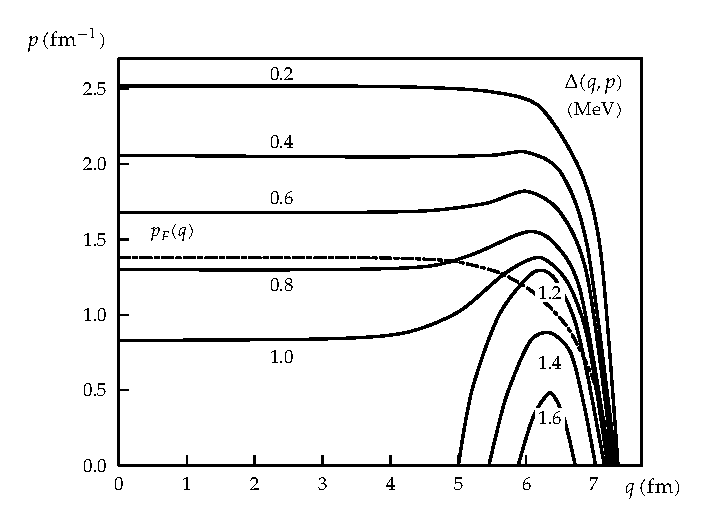
\includegraphics[width=0.7\textwidth]{pictures/13_7}
\par\end{centering}
\caption{\label{fig:13.7}图 13.7：Wigner 相空间中的中子配对能隙分布$\Delta(q,p)$，采用参数为$V_{0}=-49\,\text{MeV}$、$R_{0}=6.81\,\text{fm}$、$a=0.66\,\text{fm}$的
Woods-Saxon 势阱，中子数$N=96$。两体配对相互作用参数为$V_{0}=-28\,\text{MeV}$，$r_{0}=1.6\,\text{fm}$。}
\end{figure}

\begin{figure}[H]
\begin{centering}
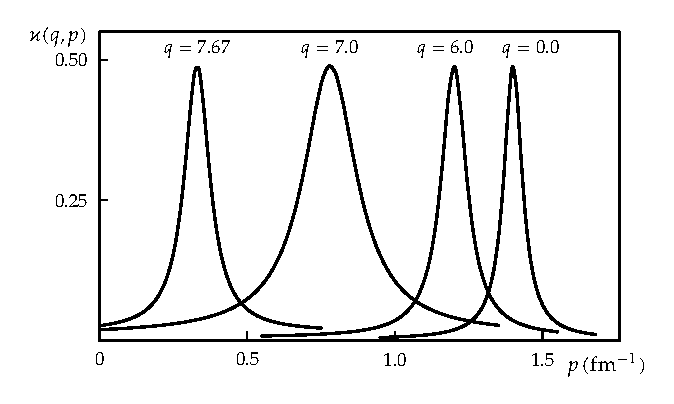
\includegraphics[width=0.65\textwidth]{pictures/13_8}
\par\end{centering}
\caption{\label{fig:13.8}图 13.8：原子核中不同空间位置$q$处的配对张量$\kappa(q,p)$（参数与图 13.7
相同）。}
\end{figure}

\begin{figure}[H]
\begin{centering}
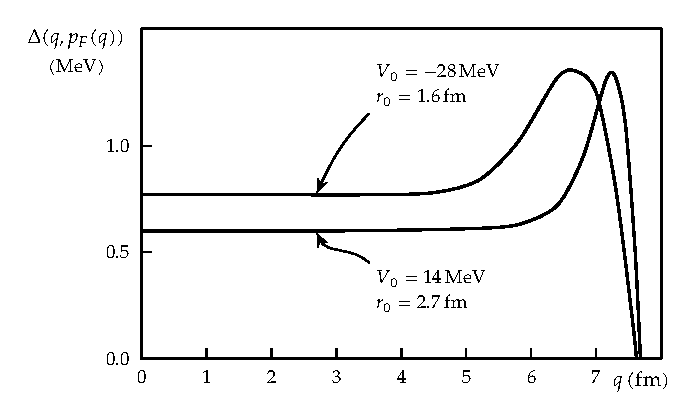
\includegraphics[width=0.65\textwidth]{pictures/13_9}
\par\end{centering}
\caption{\label{fig:13.9}图 13.9：沿局域 Fermi 面 {[}$p_{F}(q)${]} 的配对能隙分布曲线，展示了两组给出相同宏观配对能的不同核力参数的计算结果。}
\end{figure}

从图 13.7–13.9 可以清晰看出，理论计算揭示出配对能隙高度集中分布在原子核表面弥散区，表明核物理中的配对现象在本质上是一种强烈的表面效应，这对理解双核子转移反应等前沿实验过程具有至关重要的指导意义。

\section{动态情形\label{sec:13.3_=0052A8=006001=0060C5=005F62}}

至此，我们已经运用半经典方法系统研究了原子核的静态物理性质，例如核密度分布与原子核结合能。极其自然的研究延伸是将这些理论进一步推广至动力学过程，例如
RPA 与时间相关 Hartree-Fock（TDHF）理论。为此，我们必须探寻这些微观量子多体动力学理论在$\hbar\to0$时的经典极限。在动力学情形下，涌现出一系列全新的物理特征与理论课题，目前物理学界尚处于深入探索的初级阶段；因此，在这一最后章节中，我们不可能做到面面俱到，而是着重勾勒该理论的核心脉络与物理图像。

动力学情形下的基石性方程之一，乃是时间相关 Hartree-Fock 方程 (12.9) 的经典极限，它将直接引申出原子核流体动力学方程。另一条稍有不同的推导路径则是基于含时变分原理建立此类方程。此外，我们还将揭示局域动量分布在动态情形下的非球形畸变现象，并讨论半经典结论与第
8 章能量加权和规则之间的深刻内在对应。

\subsection{Boltzmann 方程\label{subsec:13.3.1_Boltzmann=0065B9=007A0B}}

为了求取 TDHF 方程 (12.9) 的经典极限，我们必须取其 Wigner 变换，这可以借助附录 D 中的算符乘积运算法则 (D.55)
来实现。由此导出的微观严格方程为 \cite{Gr46,KK76}：

\[
\frac{\partial f(\boldsymbol{q},\boldsymbol{p},t)}{\partial t}=\frac{2}{\hbar}\sin\left[\frac{\hbar}{2}\left(\boldsymbol{\nabla}^{H}_{\boldsymbol{q}}\cdot\boldsymbol{\nabla}^{f}_{\boldsymbol{p}}-\boldsymbol{\nabla}^{H}_{\boldsymbol{p}}\cdot\boldsymbol{\nabla}^{f}_{\boldsymbol{q}}\right)\right]H(\boldsymbol{q},\boldsymbol{p})f(\boldsymbol{q},\boldsymbol{p},t),
\]

式中$f(\boldsymbol{q},\boldsymbol{p},t)$是密度矩阵$\rho$的 Wigner 变换 {[}参见式
(13.41){]}，而$H(\boldsymbol{q},\boldsymbol{p})$是单体 Hartree-Fock Hamiltonian
的 Wigner 变换。为简便起见，我们暂且假定外势场是局域的，但利用式 (13.36) 很容易推广至诸如 Skyrme 型非局域势。从式
(13.68) 令$\hbar\to0$，我们极其直接地获得其经典极限：

\[
\frac{\partial f^{(0)}}{\partial t}+\frac{\boldsymbol{p}}{m}\cdot\boldsymbol{\nabla}_{\boldsymbol{q}}f^{(0)}-\boldsymbol{\nabla}_{\boldsymbol{q}}V\cdot\boldsymbol{\nabla}_{\boldsymbol{p}}f^{(0)}=0.
\]

该方程在经典统计力学中最广为人知的名称便是无碰撞 Boltzmann 方程（collisionless Boltzmann equation）\cite{UF74,Hu63}，而$(2\pi\hbar)^{-3}f^{(0)}(\boldsymbol{q},\boldsymbol{p},t)$则是相应的经典相空间分布函数。式
(13.69) 的物理内涵极其清晰直观，它无非表述了经典相空间微元内粒子流入与流出的精确平衡：第一项是分布函数的局域显含时演化率；第二项描述由于微元内粒子具有有限运动速度而引起的漂移变化；第三项则代表由于平均场力导致的粒子动量加速度改变。因此，无碰撞
Boltzmann 方程在本质上宣告了随体相空间微元内的粒子数全时间微商恒等于零：$\mathrm{d}f^{(0)}/\mathrm{d}t=0$。

这显然仅适用于独立核子在平均场势垒边缘发生弹性反射、而体系内部不存在微观真正两体直接碰撞的情形。这一无碰撞特征正深深根植于我们作为出发点的
TDHF 平均场理论。若考虑真实核子-核子微观碰撞，则分布函数方程右侧必须引入两体碰撞积分项：$\mathrm{d}f^{(0)}/\mathrm{d}t=I(f^{(0)})$，该碰撞项亦可在$\hbar\to0$极限下由我们在导出
TDHF 时所略去的两体关联函数 (12.6) 系统还原 \cite{KB62,Sch72a}。在低激发能的原子核集体运动中，由于核子在基态原子核内的平均自由程与核几何线度相当（第
4 章），在初级近似下忽略两体碰撞项是完全合理且高度成立的 \cite{KK68}。

由方程 (13.69) 出发，建立 RPA 方程的经典对应物是极其平易的，因为正如第 8.5 节所示，RPA 在本质上正是 TDHF
方程的线性化小振幅展开。取最简单的局域势拟设$V[\rho]=a\rho(\boldsymbol{q})+b\rho^{2}(\boldsymbol{q})${[}参见式
(5.99){]}，在线性化微扰下引入展开：

\[
f(\boldsymbol{q},\boldsymbol{p},t)=f^{(0)}(\boldsymbol{q},\boldsymbol{p})+\delta f(\boldsymbol{q},\boldsymbol{p},t),\quad\rho(\boldsymbol{q},t)=\rho^{(0)}(\boldsymbol{q})+\delta\rho(\boldsymbol{q},t),
\]

\[
\delta\rho(\boldsymbol{q},t)=\frac{2}{(2\pi\hbar)^{3}}\int\mathrm{d}^{3}p\,\delta f(\boldsymbol{q},\boldsymbol{p},t),\tag{13.70b}
\]

由此导出的线性化方程为：

\[
\frac{\partial\delta f}{\partial t}+\frac{\boldsymbol{p}}{m}\cdot\boldsymbol{\nabla}_{\boldsymbol{q}}\delta f-\boldsymbol{\nabla}_{\boldsymbol{q}}V^{(0)}\cdot\boldsymbol{\nabla}_{\boldsymbol{p}}\delta f-\boldsymbol{\nabla}_{\boldsymbol{p}}f^{(0)}\cdot\boldsymbol{\nabla}_{\boldsymbol{q}}\left[(a+2b\rho^{(0)})\delta\rho\right]=0.
\]

在均匀无限核物质中，式 (13.71) 的第三项严格为零，方程存在精确的解析解 \cite{KB62,No64a}。解析解显示，微扰$\delta f$在球对称平衡动量球上叠加了一个非各向同性的、呈椭球/卵形畸变且绕平衡球作四极振荡的附加分布。这种特殊的量子统计振荡模式被称为零声（zero
sound），它与经典普通流体中的流体力学第一声（普通声波，其中 Fermi 球仅作各向同性的平移与胀缩振动）具有截然不同的微观物理本质。

\subsection{由 Boltzmann 方程导出流体动力学方程\label{subsec:13.3.2_=006D41=004F53=0052A8=00529B=005B66=005BFC=0051FA}}

为了降低求解方程 (13.69) 与 (13.71) 的庞大复杂度，人们通常通过将方程乘以动量$\boldsymbol{p}$的不同幂次并对动量执行积分，将其转换为关于$f(\boldsymbol{q},\boldsymbol{p},t)$的各阶动量矩的耦合微分方程组。将方程
(13.69) 对动量分别作零阶矩、一阶矩及二阶矩积分，经过系统的代数整理，最终化为五条著名的守恒律方程：

\[
\frac{\partial\rho}{\partial t}+\sum_{i}\frac{\partial}{\partial q_{i}}(\rho u_{i})=0,
\]

\[
\rho\left(\frac{\partial u_{i}}{\partial t}+\sum_{j}u_{j}\frac{\partial u_{i}}{\partial q_{j}}\right)=-\frac{\rho}{m}\frac{\partial V}{\partial q_{i}}-\frac{1}{m}\sum_{j}\frac{\partial P_{ij}}{\partial q_{j}},
\]

\[
\frac{\partial Q}{\partial t}+\sum_{i}\frac{\partial}{\partial q_{i}}(Qu_{i})+\sum_{ij}P_{ij}D_{ij}+\sum_{i}\frac{\partial W_{i}}{\partial q_{i}}=0.
\]

在此我们引入了流体动力学中标准的核心物理量定义：

局域平均流速：$u_{i}(\boldsymbol{q},t)=\overline{p_{i}/m}$；相对平均流速的热运动速度涨落：$U_{i}(\boldsymbol{q},\boldsymbol{p},t)=p_{i}/m-u_{i}$；热动能密度：$Q(\boldsymbol{q},t)=\frac{1}{2}m\rho\overline{\boldsymbol{U}^{2}}$；压力张量（动量流密度）：$P_{ij}(\boldsymbol{q},t)=m\rho\overline{U_{i}U_{j}}$；热流密度矢量：$W_{i}(\boldsymbol{q},t)=\frac{1}{2}m\rho\overline{U_{i}\boldsymbol{U}^{2}}$；应变率张量：$D_{ij}(\boldsymbol{q},t)=\frac{1}{2}\left(\frac{\partial u_{i}}{\partial q_{j}}+\frac{\partial u_{j}}{\partial q_{i}}\right)$。

方程 (13.72)–(13.74) 严格表达了质量连续性守恒、动量平衡以及内能流平衡。然而，这组方程本身并不是闭合的，因为压力张量和热流矢量包含更高阶的动量矩未决函数。在普通流体力学与低能核多体物理中，截断闭合该级联方程组的物理假定截然不同：

(i) 在经典普通流体力学中 \cite{UF74,Hu63}，频繁的粒子剧烈碰撞使得体系在极短时间内迅速达到局域热平衡，动量分布各向同性地满足
Maxwell-Boltzmann 分布 (13.76)，从而压力张量退化为对角标量压强$P_{ij}=P\delta_{ij}$，热流$\boldsymbol{W}=0$，直接导出无粘理想流体的
Euler 方程组 (13.78)。

(ii) 在低能核物理中，核子平均自由程很大，粒子间碰撞极少。为了闭合方程组，人们假定平均场势随时间的演化足够缓慢，使得在特征单粒子周期内势场可视为近似恒定
{[}参见绝热判据 (13.79){]}。在此静态瞬时近似下，局域相空间分布函数可近似假定为瞬时 Thomas-Fermi 形式：

\[
f^{(0)}(\boldsymbol{q},\boldsymbol{p},t)=\Theta\left(\lambda-\frac{p^{2}}{2m}-V(\boldsymbol{q},t)\right).
\]

结合式 (13.80)，瞬时各向同性压力张量具有如下闭合形式：

\[
P_{ij}=\frac{\hbar^{2}}{5m}\left(3\pi^{2}\rho(\boldsymbol{q},t)\right)^{2/3}\rho(\boldsymbol{q},t)\delta_{ij}=\frac{1}{3}\tau^{\mathrm{TF}}\delta_{ij},
\]

从而实现了连续性方程 (13.72) 与动量方程 (13.73) 的初步解耦闭合。

\subsection{普通流体动力学在原子核中的应用\label{subsec:13.3.3_=006D41=004F53=0052A8=00529B=005B66=005E94=007528}}

\begin{figure}[H]
\begin{centering}
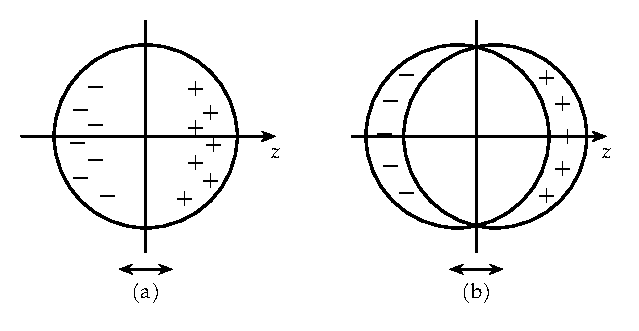
\includegraphics[width=0.7\textwidth]{pictures/13_10}
\par\end{centering}
\caption{\label{fig:13.10}图 13.10：球形核的偶极电极化模型示意图。减号代表质子缺陷（中子过剩），加号代表中子缺陷（质子过剩）。(a)
对应 Steinwedel-Jensen (SJ) 模型，(b) 对应 Goldhaber-Teller (GT) 模型。}
\end{figure}

在描述原子核巨偶极共振（GDR）等同位旋矢量激发（T=1 模式）时，历史上提出了两种著名的唯象流体动力学模型：

(1) Steinwedel-Jensen (SJ) 模型 \cite{SJ50}：假定原子核总体积与总核子密度严格保持不可压缩常数$\rho_{0}=\rho_{p}+\rho_{n}$，而质子流体与中子流体在固定的刚性核边界内发生反相相对密度振荡
{[}图 13.10(a){]}。定义相对密度差$\rho^{(1)}=\delta\rho_{p}-\delta\rho_{n}$，结合对称能变分推导出如下波动方程：

\[
\Delta\rho^{(1)}-\frac{1}{c^{2}}\frac{\partial^{2}\rho^{(1)}}{\partial t^{2}}=0,\quad c=\sqrt{\frac{2a_{\mathrm{sym}}}{m}}.
\]

在刚性核表面处无径向流出流的边界条件导出了特征偶极频率：

\[
\hbar\omega_{0}=2.08\frac{\hbar c}{R_{0}}\approx70\,A^{-1/3}\,\text{MeV}.
\]

(2) Goldhaber-Teller (GT) 模型 \cite{GT48}：假定质子流体球与中子流体球各自保持内部不可压缩，作为两个刚性刚球彼此反向平移相对振动
{[}图 13.10(b){]}。在 Tassie 表面振荡模型 \cite{Ta56a} 中，其跃迁密度完全集中在核表面弥散层，预言激发能随质量数呈$A^{-1/6}$的标度律。

\begin{figure}[H]
\begin{centering}
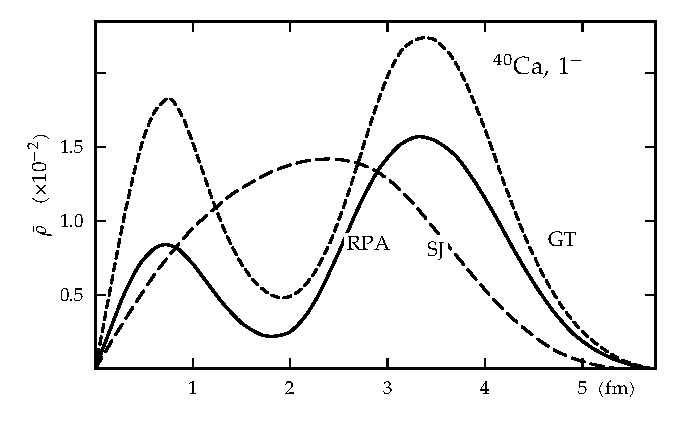
\includegraphics[width=0.65\textwidth]{pictures/13_11}
\par\end{centering}
\caption{\label{fig:13.11}图 13.11：$^{40}\text{Ca}$巨偶极态的跃迁密度对比。实线为基于微观 RPA
计算的最具集体性偶极态；虚线与点线分别代表 Goldhaber-Teller 模型与 Steinwedel-Jensen 模型的预言（引自
\cite{SR77}）。}
\end{figure}

从图 13.11 对比可见，在轻核$^{40}mathrm{Ca}$中，微观 RPA 的跃迁密度极其清晰地契合 GT 模型的表面峰化特征；而在重核中，SJ
体积振荡模式与 GT 表面位移模式则发生强烈混合 \cite{MSK77}。

\subsection{流体动力学的变分推导\label{subsec:13.3.4_=0053D8=005206=0063A8=005BFC}}

微观量子力学可以通过作用量的时间相关变分原理来严格导出。我们对多体态矢引入如下实虚部相因子分解拟设：

\[
|\Psi(t)\rangle=e^{\mathrm{i}S(t)}|\Phi_{0}(t)\rangle,
\]

假定相位算符由单粒子局域标量场决定，即对 Slater 行列式中所有单粒子轨道共享统一的空间相位$\phi_{i}(\boldsymbol{r},t)=e^{\mathrm{i}s(\boldsymbol{r},t)}\phi_{0i}(\boldsymbol{r},t)$。相应的流体速度场由相位梯度的无旋流严格给出：

\[
\boldsymbol{u}=\boldsymbol{\nabla}s.
\]

体系的总作用量积分泛函表述为经典的 Hamilton 形式，以局域密度与速度势构成正则共轭变量：

\[
I=\int\mathrm{d}t\int\mathrm{d}^{3}r\left\{ -m\dot{\rho}_{0}s-\frac{m}{2}\rho_{0}(\boldsymbol{\nabla}s)^{2}-\mathcal{E}[\rho_{0}]\right\} .
\]

变分方程直接导出连续性方程以及 Euler 形式的流体运动方程：

\[
\dot{\rho}_{0}=-\boldsymbol{\nabla}\cdot(\rho_{0}\boldsymbol{u}),
\]

\[
\frac{\partial\boldsymbol{u}}{\partial t}+(\boldsymbol{u}\cdot\boldsymbol{\nabla})\boldsymbol{u}=-\frac{1}{m}\boldsymbol{\nabla}\frac{\delta E_{\mathrm{int}}}{\delta\rho_{0}}.
\]


\subsection{密度 ρ₀ 的动量分布\label{subsec:13.3.5_=0052A8=0091CF=005206=005E03}}

在前面几节中我们数次指出：对于集体运动的流体动力学描述，将动量分布简单假定为球对称各向同性在绝大多数情况下并不成立。时间反演偶的密度矩阵$\rho_{0}$可表示为平衡密度矩阵通过厄米时间反演奇算符的变换$\rho_{0}=e^{\mathrm{i}\phi}\rho e^{-\mathrm{i}\phi}$。\footnote{这里的“静态”仅指时间以平庸的方式出现，即在每个瞬时外加约束不同，但我们均可求解一个瞬时定态（静态）Schrödinger 方程来计算$\rho_{0}${[}它不一定严格对应于该瞬时势中的基态密度
(参见第 12 章){]}。}当考虑无旋弱非局域流场时，展开至动量的一阶项：$\phi(\boldsymbol{q},\boldsymbol{p},t)=\boldsymbol{Q}(\boldsymbol{q},t)\cdot\boldsymbol{p}+\dots$。这一变换在物理几何上精确对应于将静态密度的空间坐标沿着含时位移矢量场进行局部仿射伸缩（scaling）。当原子核经历快速的集体振荡时，核子由于来不及通过频繁碰撞或能级跨越重新排布，Fermi
球将在相空间局域地发生严重的椭球形动量畸变\footnote{只有在体系激发能极高、核子平均自由程远小于核尺寸的极端高能重离子碰撞中，频繁的两体碰撞才会重新使动量分布恢复为各向同性。}。

\subsection{施加的流体动力学运动\label{subsec:13.3.6_=0065BD=0052A0=006D41=004F53=008FD0=0052A8}}

为了深入阐明动量畸变对集体激发的决定性影响，Holzwarth 和 Eckart \cite{HE78,HE79} 等学者研究了施加特定几何速度场时体系的自洽响应\footnote{另一个极其引人入胜的流场范例是所谓的扭动模（twist mode，参见第 8 章），其流场为$\boldsymbol{v}=(yz,-xz,0)$\cite{HE77,HE79}。在该模式下局域粒子数密度严格保持不变，唯有动量分布发生强烈的扭曲畸变。}。将位移场因子化为$\boldsymbol{Q}(\boldsymbol{r},t)=\alpha(t)\boldsymbol{v}(\boldsymbol{r})$，多极流场选取为：

\[
L=0:\boldsymbol{v}_{0}=\boldsymbol{r};\quad L=1:\boldsymbol{v}_{1}=\boldsymbol{\nabla}z;\quad L=2:\boldsymbol{v}_{2}=(-x,-y,2z)=\frac{1}{2}\boldsymbol{\nabla}(2z^{2}-x^{2}-y^{2}).
\]

对于四极模式（$L=2$），局域 Fermi 动量球面发生剧烈的四极形变：

\[
p^{2}_{F}(\theta,t)=p^{2}_{F}\left[1+2\alpha(t)P_{2}(\cos\theta)\right].
\]

动量球的非各向同性畸变直接给体系带来巨大的额外动能回跳弹性（恢复力常数）。动能对微扰参数$\alpha$的二阶微商给出的动能恢复力常数为：

\[
C_{T}=\left.\frac{\partial^{2}T_{\mathrm{dyn}}}{\partial\alpha^{2}}\right|_{\alpha=0}=\begin{cases}
4T_{0}, & L=0\\
0, & L=1\\
8T_{0}, & L=2
\end{cases}
\]

对于四极振动，总惯性质量参数为$B=2mA\langle r^{2}\rangle$，由此计算出的集体四极巨共振固有频率为：

\[
\hbar\Omega_{L=2}=\sqrt{\frac{4\langle T\rangle}{m\langle r^{2}\rangle}+\frac{C_{V}}{B}}\approx60\,A^{-1/3}\,\text{MeV}.
\]

这一理论预言与微观能量加权和规则 (8.167) 的精确结论惊人一致！经典普通液滴模型之所以在四极巨共振上给出完全错误的$A^{-1/2}$依赖律，其根本症结正在于彻底忽略了动态平均场边界对核子
Fermi 动量分布造成的体积各向异性畸变效应。而在偶极模式（L=1）中，由于流场与坐标无关，动量球保持刚性平移而不发生畸变；在单极呼吸模式（L=0）中，动量球各向同性均匀膨胀，普通流体力学与
Fermi 液体理论相吻合。这雄辩地证明：对于所有 L ≥ 2 的高阶多极表面集体振动，原子核必须被严格视为具有弹性切变回跳模量的量子
Fermi 液体，而非普通的经典流体。

\subsection{典型示例\label{subsec:13.3.7_=005178=00578B=00793A=004F8B}}

为了从理论上严格检验上述核流体动力学推导中所采用的基本假设，考察一个具有严格解析解的动力学微观模型是极具启发性的。假定初始核密度处于形变简谐振子势的基态，并在
t=0 时刻让其在球对称简谐振子势中开始自由演化。利用含时微观波函数 (10.89)，时间演化的密度矩阵严格表述为 \cite{BS79,SB79}：

\[
\rho(\boldsymbol{r},\boldsymbol{r}',t)=e^{\mathrm{i}\chi(\boldsymbol{r},t)}\rho_{0}(\boldsymbol{r},\boldsymbol{r}',t)e^{-\mathrm{i}\chi(\boldsymbol{r}',t)},
\]

其中瞬时流场势精确具有严格局域的形式：

\[
\chi(\boldsymbol{r},t)=\frac{m}{2}\frac{\mathrm{d}}{\mathrm{d}t}\left(\ln b_{x}x^{2}+\ln b_{y}y^{2}+\ln b_{z}z^{2}\right),
\]

且时间反演偶密度$\rho_{0}$完全由球形基态密度通过位移标度因子$\alpha_{j}(t)=-\ln b_{j}(t)$的刚性拉伸所严格给出。这一严格解析范例极其强有力地确证了核流体动力学核心假设在微观理论上的坚实立足点。
